\documentclass{standalone}
\usepackage{tikz}
\usetikzlibrary{shadows,arrows,calc}
% Define the layers to draw the diagram
\pgfdeclarelayer{background}
\pgfdeclarelayer{foreground}
\pgfsetlayers{background,main,foreground}
 
% Define block styles  
\tikzstyle{materia}=[draw, fill=blue!20, text width=6.0em, text centered,
  minimum height=1.5em,drop shadow]
\tikzstyle{element} = [materia, text width=8em, minimum width=10em,
  minimum height=3em, rounded corners, drop shadow]
\tikzstyle{texto} = [above, text width=6em, text centered]
\tikzstyle{linepart} = [draw, thick, color=black!50, -latex', dashed]
\tikzstyle{line} = [draw, thick, color=black!50, -latex']
\tikzstyle{ur}=[draw, text centered, minimum height=0.01em]
 
% Define distances for bordering
\newcommand{\blockdist}{1.3}
\newcommand{\edgedist}{1.5}

\newcommand{\textsize}{\small}

\newcommand{\element}[2]{node (p#1) [element]
  {{\textsize #2}}}
\newcommand{\elementProg}[2]{node (prog#1) [element]
  {{\texttt{\textsize #2}}}}

\newcommand{\pipe}{edge[draw=none] node [auto = false, allow upside down] {\texttt{\textsize\%$>$\%}}}

% Draw background
\newcommand{\background}[5]{%
  \begin{pgfonlayer}{background}
    % Left-top corner of the background rectangle
    \path (#1.west |- #2.north)+(-0.5,0.5) node (a1) {};
    % Right-bottom corner of the background rectanle
    \path (#3.east |- #4.south)+(+0.5,-0.25) node (a2) {};
    % Draw the background
    \path[fill=yellow!20,rounded corners, draw=black!50, dashed]
      (a1) rectangle (a2);
    \path (a1.east |- a1.south)+(0.8,-0.3) node (u1)[texto]
      {\textsize\textit{#5}};
  \end{pgfonlayer}}

\newcommand{\transreceptor}[3]{%
  \path [linepart] (#1.east) -- node [above]
    {\textsize Transreceptor #2} (#3);}

\begin{document}
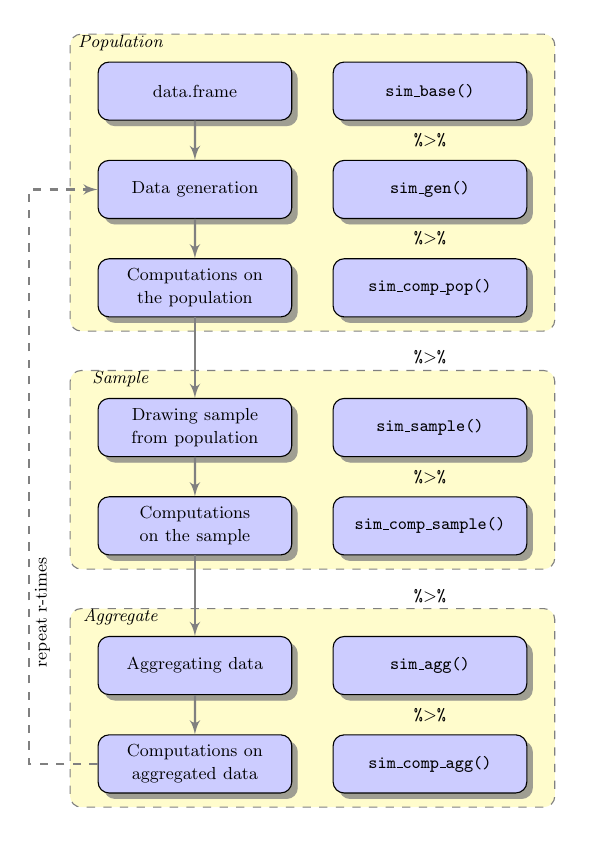
\begin{tikzpicture}[scale=0.7,transform shape]
 
  % Draw diagram elements
  % Population
  \path \element {1}{data.frame};
  \path (p1.south)+(0.0,-1.25) \element{2}{Data generation};
  \path (p2.south)+(0.0,-1.25) \element{22}{Computations on the population};
  
  \path (p1.east)+(2.5,0.0) \elementProg{1}{sim\_base()};
  \path (p2.east)+(2.5,0.0) \elementProg{2}{sim\_gen()};
  \path (p22.east)+(2.5,0.0) \elementProg{22}{sim\_comp\_pop()};
  
  % Sampling
  \path (p22.south)+(0.0,-2) \element{3}{Drawing sample from population};
  \path (p3.south)+(0.0,-1.25) \element{4}{Computations on the sample};
  
  \path (p3.east)+(2.5,0.0) \elementProg{3}{sim\_sample()};
  \path (p4.east)+(2.5,0.0) \elementProg{4}{sim\_comp\_sample()};
  
  
  % Aggregation
  \path (p4.south)+(0.0,-2) \element{5}{Aggregating data};
  \path (p5.south)+(0.0,-1.25) \element{6}{Computations on aggregated data};

  \path (p5.east)+(2.5,0.0) \elementProg{5}{sim\_agg()};
  \path (p6.east)+(2.5,0.0) \elementProg{6}{sim\_comp\_agg()};
       
  % Draw arrows between elements
  \path [line] (p1.south) -- node [above] {} (p2);
  \path [line] (p2.south) -- node [above] {} (p22);
  \path [line] (p22.south) -- node [above] {} (p3);
  \path [line] (p3.south) -- node [above] {} (p4);
  \path [line] (p4.south) -- node [above] {} (p5);
  \path [line] (p5.south) -- node [above] {} (p6);
  
  % Draw pipes
  \path [-stealth, auto] (prog1.south) \pipe (prog2.north);
  \path [-stealth, auto] (prog2.south) \pipe (prog22.north);
  \path [-stealth, auto] (prog22.south) \pipe (prog3.north);
  \path [-stealth, auto] (prog3.south) \pipe (prog4.north);
  \path [-stealth, auto] (prog4.south) \pipe (prog5.north);
  \path [-stealth, auto] (prog5.south) \pipe (prog6.north);

  % dashed lines
  \path [linepart] (p6.west) -- +(-1.25,0.0) -- ($(p2.west)+(-1.25, 0.0)$)
    -- node [above] {} (p2);

  % text
  \node [label=below:\rotatebox{90}{\textsize repeat r-times}] at ($(p6.west) + (-1.0, 4.0) $) {};
   
  \background{p1}{p1}{prog2}{p22}{Population}
  \background{p3}{p3}{prog4}{p4}{Sample}
  \background{p5}{p5}{prog6}{p6}{Aggregate}

\end{tikzpicture}
\end{document} 